\documentclass[a4paper, 11pt]{report}

%%%%%%%%%%%%%%%%%%%%%%%%%%%%%%%%%
% PACKAGE IMPORTS
%%%%%%%%%%%%%%%%%%%%%%%%%%%%%%%%%
\usepackage[tmargin=2cm,rmargin=1in,lmargin=1in,margin=0.85in,bmargin=2cm,footskip=.2in]{geometry}
\usepackage[none]{hyphenat}
\usepackage{amsmath,amsfonts,amsthm,amssymb,mathtools}
\allowdisplaybreaks
\usepackage{undertilde}
\usepackage{xfrac}
\usepackage[makeroom]{cancel}
\usepackage{mathtools}
\usepackage{bookmark}
\usepackage{enumitem}
\usepackage{kbordermatrix}
\renewcommand{\kbldelim}{(} % Change left delimiter to (
\renewcommand{\kbrdelim}{)} % Change right delimiter to )
\usepackage{hyperref,theoremref}
\hypersetup{
	pdftitle={Assignment},
	colorlinks=true, linkcolor=doc!90,
	bookmarksnumbered=true,
	bookmarksopen=true
}
\usepackage[most,many,breakable]{tcolorbox}
\usepackage{xcolor}
\usepackage{varwidth}
\usepackage{varwidth}
\usepackage{etoolbox}
%\usepackage{authblk}
\usepackage{nameref}
\usepackage{multicol,array}
\usepackage{tikz-cd}
\usepackage[ruled,vlined,linesnumbered]{algorithm2e}
\usepackage{comment} % enables the use of multi-line comments (\ifx \fi) 
\usepackage{import}
\usepackage{xifthen}
\usepackage{pdfpages}
\usepackage{svg}
\usepackage{transparent}
\usepackage{pgfplots}
\pgfplotsset{compat=1.18}
\usetikzlibrary{calc}
\usetikzlibrary{graphs}
\usetikzlibrary{graphs.standard}
% \usetikzlibrary{graphdrawing}

\newcommand\mycommfont[1]{\footnotesize\ttfamily\textcolor{blue}{#1}}
\SetCommentSty{mycommfont}
\newcommand{\incfig}[1]{%
    \def\svgwidth{\columnwidth}
    \import{./figures/}{#1.pdf_tex}
}


\usepackage{tikzsymbols}
% \renewcommand\qedsymbol{$\Laughey$}

\definecolor{commentgreen}{RGB}{2,112,10}
%%
%% Julia definition (c) 2014 Jubobs
%%
\lstdefinelanguage{Julia}%
  {morekeywords={abstract,break,case,catch,const,continue,do,else,elseif,%
      end,export,false,for,function,immutable,import,importall,if,in,%
      macro,module,otherwise,quote,return,switch,true,try,type,typealias,%
      using,while},%
   sensitive=true,%
   alsoother={$},%
   morecomment=[l]\#,%
   morecomment=[n]{\#=}{=\#},%
   morestring=[s]{"}{"},%
   morestring=[m]{'}{'},%
}[keywords,comments,strings]%

\lstset{%
    language        	= Julia,
    basicstyle      	= \ttfamily,
    keywordstyle    	= \bfseries\color{blue},
    stringstyle     	= \color{magenta},
    commentstyle    	= \color{commentgreen},
    showstringspaces	= false,
		numbers						= left,
		tabsize						= 4,
}

\definecolor{stringyellow}{RGB}{227, 78, 48}
%% 
%% Shamelessly stolen from Vivi on Stackoverflow
%% https://tex.stackexchange.com/questions/75116/what-can-i-use-to-typeset-matlab-code-in-my-document
%%
\lstset{language=Matlab,%
    %basicstyle=\color{red},
    breaklines=true,%
    morekeywords={matlab2tikz},
		morekeywords={subtitle}
    keywordstyle=\color{blue},%
    morekeywords=[2]{1}, keywordstyle=[2]{\color{black}},
    identifierstyle=\color{black},%
    stringstyle=\color{stringyellow},
    commentstyle=\color{commentgreen},%
    showstringspaces=false,%without this there will be a symbol in the places where there is a space
    numbers=left,%
		firstnumber=1,
    % numberstyle={\tiny \color{black}},% size of the numbers
    % numbersep=9pt, % this defines how far the numbers are from the text
    emph=[1]{for,end,break},emphstyle=[1]\color{red}, %some words to emphasise
    %emph=[2]{word1,word2}, emphstyle=[2]{style},    
}

%% 
%% Shamelessly stolen from egreg on Stackoverflow
%% https://tex.stackexchange.com/questions/280681/how-to-have-multiple-lines-of-intertext-within-align-environment
%%
\newlength{\normalparindent}
\AtBeginDocument{\setlength{\normalparindent}{\parindent}}
\newcommand{\longintertext}[1]{%
  \intertext{%
    \parbox{\linewidth}{%
      \setlength{\parindent}{\normalparindent}
      \noindent#1%
    }%
  }%
}

%\usepackage{import}
%\usepackage{xifthen}
%\usepackage{pdfpages}
%\usepackage{transparent}

%%%%%%%%%%%%%%%%%%%%%%%%%%%%%%
% SELF MADE COLORS
%%%%%%%%%%%%%%%%%%%%%%%%%%%%%%
\definecolor{myg}{RGB}{56, 140, 70}
\definecolor{myb}{RGB}{45, 111, 177}
\definecolor{myr}{RGB}{199, 68, 64}
\definecolor{mytheorembg}{HTML}{F2F2F9}
\definecolor{mytheoremfr}{HTML}{00007B}
\definecolor{mylenmabg}{HTML}{FFFAF8}
\definecolor{mylenmafr}{HTML}{983b0f}
\definecolor{mypropbg}{HTML}{f2fbfc}
\definecolor{mypropfr}{HTML}{191971}
\definecolor{myexamplebg}{HTML}{F2FBF8}
\definecolor{myexamplefr}{HTML}{88D6D1}
\definecolor{myexampleti}{HTML}{2A7F7F}
\definecolor{mydefinitbg}{HTML}{E5E5FF}
\definecolor{mydefinitfr}{HTML}{3F3FA3}
\definecolor{notesgreen}{RGB}{0,162,0}
\definecolor{myp}{RGB}{197, 92, 212}
\definecolor{mygr}{HTML}{2C3338}
\definecolor{myred}{RGB}{127,0,0}
\definecolor{myyellow}{RGB}{169,121,69}
\definecolor{myexercisebg}{HTML}{F2FBF8}
\definecolor{myexercisefg}{HTML}{88D6D1}

%%%%%%%%%%%%%%%%%%%%%%%%%%%%
% TCOLORBOX SETUPS
%%%%%%%%%%%%%%%%%%%%%%%%%%%%
\setlength{\parindent}{0pt}

%================================
% THEOREM BOX
%================================
\tcbuselibrary{theorems,skins,hooks}
\newtcbtheorem[number within=section]{Theorem}{Theorem}
{%
	enhanced,
	breakable,
	colback = mytheorembg,
	frame hidden,
	boxrule = 0sp,
	borderline west = {2pt}{0pt}{mytheoremfr},
	sharp corners,
	detach title,
	before upper = \tcbtitle\par\smallskip,
	coltitle = mytheoremfr,
	fonttitle = \bfseries\sffamily,
	description font = \mdseries,
	separator sign none,
	segmentation style={solid, mytheoremfr},
}
{th}

\tcbuselibrary{theorems,skins,hooks}
\newtcbtheorem[number within=chapter]{theorem}{Theorem}
{%
	enhanced,
	breakable,
	colback = mytheorembg,
	frame hidden,
	boxrule = 0sp,
	borderline west = {2pt}{0pt}{mytheoremfr},
	sharp corners,
	detach title,
	before upper = \tcbtitle\par\smallskip,
	coltitle = mytheoremfr,
	fonttitle = \bfseries\sffamily,
	description font = \mdseries,
	separator sign none,
	segmentation style={solid, mytheoremfr},
}
{th}


\tcbuselibrary{theorems,skins,hooks}
\newtcolorbox{Theoremcon}
{%
	enhanced
	,breakable
	,colback = mytheorembg
	,frame hidden
	,boxrule = 0sp
	,borderline west = {2pt}{0pt}{mytheoremfr}
	,sharp corners
	,description font = \mdseries
	,separator sign none
}

%================================
% Corollery
%================================
\tcbuselibrary{theorems,skins,hooks}
\newtcbtheorem[number within=section]{Corollary}{Corollary}
{%
	enhanced
	,breakable
	,colback = myp!10
	,frame hidden
	,boxrule = 0sp
	,borderline west = {2pt}{0pt}{myp!85!black}
	,sharp corners
	,detach title
	,before upper = \tcbtitle\par\smallskip
	,coltitle = myp!85!black
	,fonttitle = \bfseries\sffamily
	,description font = \mdseries
	,separator sign none
	,segmentation style={solid, myp!85!black}
}
{th}
\tcbuselibrary{theorems,skins,hooks}
\newtcbtheorem[number within=chapter]{corollary}{Corollary}
{%
	enhanced
	,breakable
	,colback = myp!10
	,frame hidden
	,boxrule = 0sp
	,borderline west = {2pt}{0pt}{myp!85!black}
	,sharp corners
	,detach title
	,before upper = \tcbtitle\par\smallskip
	,coltitle = myp!85!black
	,fonttitle = \bfseries\sffamily
	,description font = \mdseries
	,separator sign none
	,segmentation style={solid, myp!85!black}
}
{th}

%================================
% LENMA
%================================
\tcbuselibrary{theorems,skins,hooks}
\newtcbtheorem[number within=section]{Lenma}{Lenma}
{%
	enhanced,
	breakable,
	colback = mylenmabg,
	frame hidden,
	boxrule = 0sp,
	borderline west = {2pt}{0pt}{mylenmafr},
	sharp corners,
	detach title,
	before upper = \tcbtitle\par\smallskip,
	coltitle = mylenmafr,
	fonttitle = \bfseries\sffamily,
	description font = \mdseries,
	separator sign none,
	segmentation style={solid, mylenmafr},
}
{th}

\tcbuselibrary{theorems,skins,hooks}
\newtcbtheorem[number within=chapter]{lenma}{Lenma}
{%
	enhanced,
	breakable,
	colback = mylenmabg,
	frame hidden,
	boxrule = 0sp,
	borderline west = {2pt}{0pt}{mylenmafr},
	sharp corners,
	detach title,
	before upper = \tcbtitle\par\smallskip,
	coltitle = mylenmafr,
	fonttitle = \bfseries\sffamily,
	description font = \mdseries,
	separator sign none,
	segmentation style={solid, mylenmafr},
}
{th}

%================================
% PROPOSITION
%================================
\tcbuselibrary{theorems,skins,hooks}
\newtcbtheorem[number within=section]{Prop}{Proposition}
{%
	enhanced,
	breakable,
	colback = mypropbg,
	frame hidden,
	boxrule = 0sp,
	borderline west = {2pt}{0pt}{mypropfr},
	sharp corners,
	detach title,
	before upper = \tcbtitle\par\smallskip,
	coltitle = mypropfr,
	fonttitle = \bfseries\sffamily,
	description font = \mdseries,
	separator sign none,
	segmentation style={solid, mypropfr},
}
{th}

\tcbuselibrary{theorems,skins,hooks}
\newtcbtheorem[number within=chapter]{prop}{Proposition}
{%
	enhanced,
	breakable,
	colback = mypropbg,
	frame hidden,
	boxrule = 0sp,
	borderline west = {2pt}{0pt}{mypropfr},
	sharp corners,
	detach title,
	before upper = \tcbtitle\par\smallskip,
	coltitle = mypropfr,
	fonttitle = \bfseries\sffamily,
	description font = \mdseries,
	separator sign none,
	segmentation style={solid, mypropfr},
}
{th}

%================================
% CLAIM
%================================
\tcbuselibrary{theorems,skins,hooks}
\newtcbtheorem[number within=section]{claim}{Claim}
{%
	enhanced
	,breakable
	,colback = myg!10
	,frame hidden
	,boxrule = 0sp
	,borderline west = {2pt}{0pt}{myg}
	,sharp corners
	,detach title
	,before upper = \tcbtitle\par\smallskip
	,coltitle = myg!85!black
	,fonttitle = \bfseries\sffamily
	,description font = \mdseries
	,separator sign none
	,segmentation style={solid, myg!85!black}
}
{th}

%================================
% Exercise
%================================
\tcbuselibrary{theorems,skins,hooks}
\newtcbtheorem[number within=section]{Exercise}{Exercise}
{%
	enhanced,
	breakable,
	colback = myexercisebg,
	frame hidden,
	boxrule = 0sp,
	borderline west = {2pt}{0pt}{myexercisefg},
	sharp corners,
	detach title,
	before upper = \tcbtitle\par\smallskip,
	coltitle = myexercisefg,
	fonttitle = \bfseries\sffamily,
	description font = \mdseries,
	separator sign none,
	segmentation style={solid, myexercisefg},
}
{th}

\tcbuselibrary{theorems,skins,hooks}
\newtcbtheorem[number within=chapter]{exercise}{Exercise}
{%
	enhanced,
	breakable,
	colback = myexercisebg,
	frame hidden,
	boxrule = 0sp,
	borderline west = {2pt}{0pt}{myexercisefg},
	sharp corners,
	detach title,
	before upper = \tcbtitle\par\smallskip,
	coltitle = myexercisefg,
	fonttitle = \bfseries\sffamily,
	description font = \mdseries,
	separator sign none,
	segmentation style={solid, myexercisefg},
}
{th}

%================================
% EXAMPLE BOX
%================================
\newtcbtheorem[number within=section]{Example}{Example}
{%
	colback = myexamplebg
	,breakable
	,colframe = myexamplefr
	,coltitle = myexampleti
	,boxrule = 1pt
	,sharp corners
	,detach title
	,before upper=\tcbtitle\par\smallskip
	,fonttitle = \bfseries
	,description font = \mdseries
	,separator sign none
	,description delimiters parenthesis
}
{ex}

\newtcbtheorem[number within=chapter]{example}{Example}
{%
	colback = myexamplebg
	,breakable
	,colframe = myexamplefr
	,coltitle = myexampleti
	,boxrule = 1pt
	,sharp corners
	,detach title
	,before upper=\tcbtitle\par\smallskip
	,fonttitle = \bfseries
	,description font = \mdseries
	,separator sign none
	,description delimiters parenthesis
}
{ex}

%================================
% DEFINITION BOX
%================================
\newtcbtheorem[number within=section]{Definition}{Definition}{enhanced,
	before skip=2mm,after skip=2mm, colback=red!5,colframe=red!80!black,boxrule=0.5mm,
	attach boxed title to top left={xshift=1cm,yshift*=1mm-\tcboxedtitleheight}, varwidth boxed title*=-3cm,
	boxed title style={frame code={
					\path[fill=tcbcolback]
					([yshift=-1mm,xshift=-1mm]frame.north west)
					arc[start angle=0,end angle=180,radius=1mm]
					([yshift=-1mm,xshift=1mm]frame.north east)
					arc[start angle=180,end angle=0,radius=1mm];
					\path[left color=tcbcolback!60!black,right color=tcbcolback!60!black,
						middle color=tcbcolback!80!black]
					([xshift=-2mm]frame.north west) -- ([xshift=2mm]frame.north east)
					[rounded corners=1mm]-- ([xshift=1mm,yshift=-1mm]frame.north east)
					-- (frame.south east) -- (frame.south west)
					-- ([xshift=-1mm,yshift=-1mm]frame.north west)
					[sharp corners]-- cycle;
				},interior engine=empty,
		},
	fonttitle=\bfseries,
	title={#2},#1}{def}
\newtcbtheorem[number within=chapter]{definition}{Definition}{enhanced,
	before skip=2mm,after skip=2mm, colback=red!5,colframe=red!80!black,boxrule=0.5mm,
	attach boxed title to top left={xshift=1cm,yshift*=1mm-\tcboxedtitleheight}, varwidth boxed title*=-3cm,
	boxed title style={frame code={
					\path[fill=tcbcolback]
					([yshift=-1mm,xshift=-1mm]frame.north west)
					arc[start angle=0,end angle=180,radius=1mm]
					([yshift=-1mm,xshift=1mm]frame.north east)
					arc[start angle=180,end angle=0,radius=1mm];
					\path[left color=tcbcolback!60!black,right color=tcbcolback!60!black,
						middle color=tcbcolback!80!black]
					([xshift=-2mm]frame.north west) -- ([xshift=2mm]frame.north east)
					[rounded corners=1mm]-- ([xshift=1mm,yshift=-1mm]frame.north east)
					-- (frame.south east) -- (frame.south west)
					-- ([xshift=-1mm,yshift=-1mm]frame.north west)
					[sharp corners]-- cycle;
				},interior engine=empty,
		},
	fonttitle=\bfseries,
	title={#2},#1}{def}

%================================
% Solution BOX
%================================
\makeatletter
\newtcbtheorem{question}{Question}{enhanced,
	breakable,
	colback=white,
	colframe=myb!80!black,
	attach boxed title to top left={yshift*=-\tcboxedtitleheight},
	fonttitle=\bfseries,
	title={#2},
	boxed title size=title,
	boxed title style={%
			sharp corners,
			rounded corners=northwest,
			colback=tcbcolframe,
			boxrule=0pt,
		},
	underlay boxed title={%
			\path[fill=tcbcolframe] (title.south west)--(title.south east)
			to[out=0, in=180] ([xshift=5mm]title.east)--
			(title.center-|frame.east)
			[rounded corners=\kvtcb@arc] |-
			(frame.north) -| cycle;
		},
	#1
}{def}
\makeatother

%================================
% SOLUTION BOX
%================================
\makeatletter
\newtcolorbox{solution}{enhanced,
	breakable,
	colback=white,
	colframe=myg!80!black,
	attach boxed title to top left={yshift*=-\tcboxedtitleheight},
	title=Solution,
	boxed title size=title,
	boxed title style={%
			sharp corners,
			rounded corners=northwest,
			colback=tcbcolframe,
			boxrule=0pt,
		},
	underlay boxed title={%
			\path[fill=tcbcolframe] (title.south west)--(title.south east)
			to[out=0, in=180] ([xshift=5mm]title.east)--
			(title.center-|frame.east)
			[rounded corners=\kvtcb@arc] |-
			(frame.north) -| cycle;
		},
}
\makeatother

%================================
% Question BOX
%================================
\makeatletter
\newtcbtheorem{qstion}{Question}{enhanced,
	breakable,
	colback=white,
	colframe=mygr,
	attach boxed title to top left={yshift*=-\tcboxedtitleheight},
	fonttitle=\bfseries,
	title={#2},
	boxed title size=title,
	boxed title style={%
			sharp corners,
			rounded corners=northwest,
			colback=tcbcolframe,
			boxrule=0pt,
		},
	underlay boxed title={%
			\path[fill=tcbcolframe] (title.south west)--(title.south east)
			to[out=0, in=180] ([xshift=5mm]title.east)--
			(title.center-|frame.east)
			[rounded corners=\kvtcb@arc] |-
			(frame.north) -| cycle;
		},
	#1
}{def}
\makeatother

\newtcbtheorem[number within=chapter]{wconc}{Wrong Concept}{
	breakable,
	enhanced,
	colback=white,
	colframe=myr,
	arc=0pt,
	outer arc=0pt,
	fonttitle=\bfseries\sffamily\large,
	colbacktitle=myr,
	attach boxed title to top left={},
	boxed title style={
			enhanced,
			skin=enhancedfirst jigsaw,
			arc=3pt,
			bottom=0pt,
			interior style={fill=myr}
		},
	#1
}{def}

%================================
% NOTE BOX
%================================
\usetikzlibrary{arrows,calc,shadows.blur}
\tcbuselibrary{skins}
\newtcolorbox{note}[1][]{%
	enhanced jigsaw,
	colback=gray!20!white,%
	colframe=gray!80!black,
	size=small,
	boxrule=1pt,
	title=\textbf{Note:-},
	halign title=flush center,
	coltitle=black,
	breakable,
	drop shadow=black!50!white,
	attach boxed title to top left={xshift=1cm,yshift=-\tcboxedtitleheight/2,yshifttext=-\tcboxedtitleheight/2},
	minipage boxed title=1.5cm,
	boxed title style={%
			colback=white,
			size=fbox,
			boxrule=1pt,
			boxsep=2pt,
			underlay={%
					\coordinate (dotA) at ($(interior.west) + (-0.5pt,0)$);
					\coordinate (dotB) at ($(interior.east) + (0.5pt,0)$);
					\begin{scope}
						\clip (interior.north west) rectangle ([xshift=3ex]interior.east);
						\filldraw [white, blur shadow={shadow opacity=60, shadow yshift=-.75ex}, rounded corners=2pt] (interior.north west) rectangle (interior.south east);
					\end{scope}
					\begin{scope}[gray!80!black]
						\fill (dotA) circle (2pt);
						\fill (dotB) circle (2pt);
					\end{scope}
				},
		},
	#1,
}

%%%%%%%%%%%%%%%%%%%%%%%%%%%%%%
% SELF MADE COMMANDS
%%%%%%%%%%%%%%%%%%%%%%%%%%%%%%
\newcommand{\thm}[2]{\begin{Theorem}{#1}{}#2\end{Theorem}}
\newcommand{\cor}[2]{\begin{Corollary}{#1}{}#2\end{Corollary}}
\newcommand{\mlenma}[2]{\begin{Lenma}{#1}{}#2\end{Lenma}}
\newcommand{\mprop}[2]{\begin{Prop}{#1}{}#2\end{Prop}}
\newcommand{\clm}[3]{\begin{claim}{#1}{#2}#3\end{claim}}
\newcommand{\wc}[2]{\begin{wconc}{#1}{}\setlength{\parindent}{1cm}#2\end{wconc}}
\newcommand{\thmcon}[1]{\begin{Theoremcon}{#1}\end{Theoremcon}}
\newcommand{\ex}[2]{\begin{Example}{#1}{}#2\end{Example}}
\newcommand{\dfn}[2]{\begin{Definition}[colbacktitle=red!75!black]{#1}{}#2\end{Definition}}
\newcommand{\dfnc}[2]{\begin{definition}[colbacktitle=red!75!black]{#1}{}#2\end{definition}}
\newcommand{\qs}[2]{\begin{question}{#1}{}#2\end{question}}
\newcommand{\pf}[2]{\begin{myproof}[#1]#2\end{myproof}}
\newcommand{\nt}[1]{\begin{note}#1\end{note}}

\newcommand*\circled[1]{\tikz[baseline=(char.base)]{
		\node[shape=circle,draw,inner sep=1pt] (char) {#1};}}
\newcommand\getcurrentref[1]{%
	\ifnumequal{\value{#1}}{0}
	{??}
	{\the\value{#1}}%
}
\newcommand{\getCurrentSectionNumber}{\getcurrentref{section}}
\newenvironment{myproof}[1][\proofname]{%
	\proof[\bfseries #1: ]%
}{\endproof}

\newcommand{\mclm}[2]{\begin{myclaim}[#1]#2\end{myclaim}}
\newenvironment{myclaim}[1][\claimname]{\proof[\bfseries #1: ]}{}

\newcounter{mylabelcounter}

\makeatletter
\newcommand{\setword}[2]{%
	\phantomsection
	#1\def\@currentlabel{\unexpanded{#1}}\label{#2}%
}
\makeatother

\tikzset{
	symbol/.style={
			draw=none,
			every to/.append style={
					edge node={node [sloped, allow upside down, auto=false]{$#1$}}}
		}
}

% deliminators
\DeclarePairedDelimiter{\abs}{\lvert}{\rvert}
\DeclarePairedDelimiter{\norm}{\lVert}{\rVert}

\DeclarePairedDelimiter{\ceil}{\lceil}{\rceil}
\DeclarePairedDelimiter{\floor}{\lfloor}{\rfloor}
\DeclarePairedDelimiter{\round}{\lfloor}{\rceil}

\newsavebox\diffdbox
\newcommand{\slantedromand}{{\mathpalette\makesl{d}}}
\newcommand{\makesl}[2]{%
\begingroup
\sbox{\diffdbox}{$\mathsurround=0pt#1\mathrm{#2}$}%
\pdfsave
\pdfsetmatrix{1 0 0.2 1}%
\rlap{\usebox{\diffdbox}}%
\pdfrestore
\hskip\wd\diffdbox
\endgroup
}
\newcommand{\dd}[1][]{\ensuremath{\mathop{}\!\ifstrempty{#1}{%
\slantedromand\@ifnextchar^{\hspace{0.2ex}}{\hspace{0.1ex}}}%
{\slantedromand\hspace{0.2ex}^{#1}}}}
\ProvideDocumentCommand\dv{o m g}{%
  \ensuremath{%
    \IfValueTF{#3}{%
      \IfNoValueTF{#1}{%
        \frac{\dd #2}{\dd #3}%
      }{%
        \frac{\dd^{#1} #2}{\dd #3^{#1}}%
      }%
    }{%
      \IfNoValueTF{#1}{%
        \frac{\dd}{\dd #2}%
      }{%
        \frac{\dd^{#1}}{\dd #2^{#1}}%
      }%
    }%
  }%
}
\providecommand*{\pdv}[3][]{\frac{\partial^{#1}#2}{\partial#3^{#1}}}
%  - others
\DeclareMathOperator{\Lap}{\mathcal{L}}
\DeclareMathOperator{\Var}{Var} % varience
\DeclareMathOperator{\Cov}{Cov} % covarience
\DeclareMathOperator{\E}{E} % expected

% Since the amsthm package isn't loaded

% I dot not prefer the slanted \leq ;P
% % I prefer the slanted \leq
% \let\oldleq\leq % save them in case they're every wanted
% \let\oldgeq\geq
% \renewcommand{\leq}{\leqslant}
% \renewcommand{\geq}{\geqslant}

% % redefine matrix env to allow for alignment, use r as default
% \renewcommand*\env@matrix[1][r]{\hskip -\arraycolsep
%     \let\@ifnextchar\new@ifnextchar
%     \array{*\c@MaxMatrixCols #1}}

%\usepackage{framed}
%\usepackage{titletoc}
%\usepackage{etoolbox}
%\usepackage{lmodern}

%\patchcmd{\tableofcontents}{\contentsname}{\sffamily\contentsname}{}{}

%\renewenvironment{leftbar}
%{\def\FrameCommand{\hspace{6em}%
%		{\color{myyellow}\vrule width 2pt depth 6pt}\hspace{1em}}%
%	\MakeFramed{\parshape 1 0cm \dimexpr\textwidth-6em\relax\FrameRestore}\vskip2pt%
%}
%{\endMakeFramed}

%\titlecontents{chapter}
%[0em]{\vspace*{2\baselineskip}}
%{\parbox{4.5em}{%
%		\hfill\Huge\sffamily\bfseries\color{myred}\thecontentspage}%
%	\vspace*{-2.3\baselineskip}\leftbar\textsc{\small\chaptername~\thecontentslabel}\\\sffamily}
%{}{\endleftbar}
%\titlecontents{section}
%[8.4em]
%{\sffamily\contentslabel{3em}}{}{}
%{\hspace{0.5em}\nobreak\itshape\color{myred}\contentspage}
%\titlecontents{subsection}
%[8.4em]
%{\sffamily\contentslabel{3em}}{}{}  
%{\hspace{0.5em}\nobreak\itshape\color{myred}\contentspage}

%%%%%%%%%%%%%%%%%%%%%%%%%%%%%%%%%%%%%%%%%%%
% TABLE OF CONTENTS
%%%%%%%%%%%%%%%%%%%%%%%%%%%%%%%%%%%%%%%%%%%
\usepackage{tikz}
\definecolor{doc}{RGB}{0,60,110}
\usepackage{titletoc}
\contentsmargin{0cm}
\titlecontents{chapter}[3.7pc]
{\addvspace{30pt}%
	\begin{tikzpicture}[remember picture, overlay]%
		\draw[fill=doc!60,draw=doc!60] (-7,-.1) rectangle (-0.9,.5);%
		\pgftext[left,x=-3.5cm,y=0.2cm]{\color{white}\Large\sc\bfseries Chapter\ \thecontentslabel};%
	\end{tikzpicture}\color{doc!60}\large\sc\bfseries}%
{}
{}
{\;\titlerule\;\large\sc\bfseries Page \thecontentspage
	\begin{tikzpicture}[remember picture, overlay]
		\draw[fill=doc!60,draw=doc!60] (2pt,0) rectangle (4,0.1pt);
	\end{tikzpicture}}%
\titlecontents{section}[3.7pc]
{\addvspace{2pt}}
{\contentslabel[\thecontentslabel]{2pc}}
{}
{\hfill\small \thecontentspage}
[]
\titlecontents*{subsection}[3.7pc]
{\addvspace{-1pt}\small}
{}
{}
{\ --- \small\thecontentspage}
[ \textbullet\ ][]

\makeatletter
\renewcommand{\tableofcontents}{%
	\chapter*{%
	  \vspace*{-20\p@}%
	  \begin{tikzpicture}[remember picture, overlay]%
		  \pgftext[right,x=15cm,y=0.2cm]{\color{doc!60}\Huge\sc\bfseries \contentsname};%
		  \draw[fill=doc!60,draw=doc!60] (13,-.75) rectangle (20,1);%
		  \clip (13,-.75) rectangle (20,1);
		  \pgftext[right,x=15cm,y=0.2cm]{\color{white}\Huge\sc\bfseries \contentsname};%
	  \end{tikzpicture}}%
	\@starttoc{toc}}
\makeatother

\newcommand{\inv}{^{-1}}
\newcommand{\opname}{\operatorname}
\newcommand{\surjto}{\twoheadrightarrow}
% \newcommand{\injto}{\hookrightarrow}
\newcommand{\injto}{\rightarrowtail}
\newcommand{\bijto}{\leftrightarrow}

\newcommand{\liff}{\leftrightarrow}
\newcommand{\notliff}{\mathrel{\ooalign{$\leftrightarrow$\cr\hidewidth$/$\hidewidth}}}
\newcommand{\lthen}{\rightarrow}
\let\varlnot\lnot
\newcommand{\ordsim}{\mathord{\sim}}
\renewcommand{\lnot}{\ordsim}
\newcommand{\lxor}{\oplus}
\newcommand{\lnand}{\barwedge}
\newcommand{\divs}{\mathrel{\mid}}
\newcommand{\ndivs}{\mathrel{\nmid}}
\def\contra{\tikz[baseline, x=0.22em, y=0.22em, line width=0.032em]\draw (0,2.83)--(2.83,0) (0.71,3.54)--(3.54,0.71) (0,0.71)--(2.83,3.54) (0.71,0)--(3.54,2.83);}

\newcommand{\On}{\mathrm{On}} % ordinals
\DeclareMathOperator{\img}{im} % Image
\DeclareMathOperator{\Img}{Im} % Image
\DeclareMathOperator{\coker}{coker} % Cokernel
\DeclareMathOperator{\Coker}{Coker} % Cokernel
\DeclareMathOperator{\Ker}{Ker} % Kernel
\DeclareMathOperator{\rank}{rank}
\DeclareMathOperator{\Spec}{Spec} % spectrum
\DeclareMathOperator{\Tr}{Tr} % trace
\DeclareMathOperator{\pr}{pr} % projection
\DeclareMathOperator{\ext}{ext} % extension
\DeclareMathOperator{\pred}{pred} % predecessor
\DeclareMathOperator{\dom}{dom} % domain
\DeclareMathOperator{\ran}{ran} % range
\DeclareMathOperator{\Hom}{Hom} % homomorphism
\DeclareMathOperator{\Mor}{Mor} % morphisms
\DeclareMathOperator{\End}{End} % endomorphism
\DeclareMathOperator{\Span}{span}
\newcommand{\Mod}{\mathbin{\mathrm{mod}}}

\newcommand{\eps}{\epsilon}
\newcommand{\veps}{\varepsilon}
\newcommand{\ol}{\overline}
\newcommand{\ul}{\underline}
\newcommand{\wt}{\widetilde}
\newcommand{\wh}{\widehat}
\newcommand{\ut}{\utilde}
\newcommand{\unit}[1]{\ut{\hat{#1}}}
\newcommand{\emp}{\varnothing}

\newcommand{\vocab}[1]{\textbf{\color{blue} #1}}
\providecommand{\half}{\frac{1}{2}}
\newcommand{\dang}{\measuredangle} %% Directed angle
\newcommand{\ray}[1]{\overrightarrow{#1}}
\newcommand{\seg}[1]{\overline{#1}}
\newcommand{\arc}[1]{\wideparen{#1}}
\DeclareMathOperator{\cis}{cis}
\DeclareMathOperator*{\lcm}{lcm}
\DeclareMathOperator*{\argmin}{arg min}
\DeclareMathOperator*{\argmax}{arg max}
\newcommand{\cycsum}{\sum_{\mathrm{cyc}}}
\newcommand{\symsum}{\sum_{\mathrm{sym}}}
\newcommand{\cycprod}{\prod_{\mathrm{cyc}}}
\newcommand{\symprod}{\prod_{\mathrm{sym}}}
\newcommand{\parinn}{\setlength{\parindent}{1cm}}
\newcommand{\parinf}{\setlength{\parindent}{0cm}}
% \newcommand{\norm}{\|\cdot\|}
\newcommand{\inorm}{\norm_{\infty}}
\newcommand{\opensets}{\{V_{\alpha}\}_{\alpha\in I}}
\newcommand{\oset}{V_{\alpha}}
\newcommand{\opset}[1]{V_{\alpha_{#1}}}
\newcommand{\lub}{\text{lub}}
\newcommand{\lm}{\lambda}
\newcommand{\uin}{\mathbin{\rotatebox[origin=c]{90}{$\in$}}}
\newcommand{\usubset}{\mathbin{\rotatebox[origin=c]{90}{$\subset$}}}
\newcommand{\lt}{\left}
\newcommand{\rt}{\right}
\newcommand{\bs}[1]{\boldsymbol{#1}}
\newcommand{\exs}{\exists}
\newcommand{\st}{\strut}
\newcommand{\dps}[1]{\displaystyle{#1}}

\newcommand{\sol}{\textbf{\textit{Solution:}} }
\newcommand{\solve}[1]{\textbf{\textit{Solution: }} #1 \qed}
% \newcommand{\proof}{\underline{\textit{proof:}}\\}

\DeclareMathOperator{\sech}{sech}
\DeclareMathOperator{\csch}{csch}
\DeclareMathOperator{\arcsec}{arcsec}
\DeclareMathOperator{\arccsc}{arccsc}
\DeclareMathOperator{\arccot}{arccot}
\DeclareMathOperator{\arsinh}{arsinh}
\DeclareMathOperator{\arcosh}{arcosh}
\DeclareMathOperator{\artanh}{artanh}
\DeclareMathOperator{\arcsch}{arcsch}
\DeclareMathOperator{\arsech}{arsech}
\DeclareMathOperator{\arcoth}{arcoth}

\newcommand{\sinx}{\sin x}          \newcommand{\arcsinx}{\arcsin x}    
\newcommand{\cosx}{\cos x}          \newcommand{\arccosx}{\arccosx}
\newcommand{\tanx}{\tan x}          \newcommand{\arctanx}{\arctan x}
\newcommand{\cscx}{\csc x}          \newcommand{\arccscx}{\arccsc x}
\newcommand{\secx}{\sec x}          \newcommand{\arcsecx}{\arcsec x}
\newcommand{\cotx}{\cot x}          \newcommand{\arccotx}{\arccot x}
\newcommand{\sinhx}{\sinh x}          \newcommand{\arsinhx}{\arsinh x}
\newcommand{\coshx}{\cosh x}          \newcommand{\arcoshx}{\arcosh x}
\newcommand{\tanhx}{\tanh x}          \newcommand{\artanhx}{\artanh x}
\newcommand{\cschx}{\csch x}          \newcommand{\arcschx}{\arcsch x}
\newcommand{\sechx}{\sech x}          \newcommand{\arsechx}{\arsech x}
\newcommand{\cothx}{\coth x}          \newcommand{\arcothx}{\arcoth x}
\newcommand{\lnx}{\ln x}
\newcommand{\expx}{\exp x}

\newcommand{\Theom}{\textbf{Theorem. }}
\newcommand{\Lemma}{\textbf{Lemma. }}
\newcommand{\Corol}{\textbf{Corollary. }}
\newcommand{\Remar}{\textit{Remark. }}
\newcommand{\Defin}[1]{\textbf{Definition} (#1).}
\newcommand{\Claim}{\textbf{Claim. }}
\newcommand{\Propo}{\textbf{Proposition. }}

\newcommand{\lb}{\left(}
\newcommand{\rb}{\right)}
\newcommand{\lbr}{\left\lbrace}
\newcommand{\rbr}{\right\rbrace}
\newcommand{\lsb}{\left[}
\newcommand{\rsb}{\right]}
\newcommand{\bracks}[1]{\lb #1 \rb}
\newcommand{\braces}[1]{\lbr #1 \rbr}
\newcommand{\suchthat}{\medspace\middle|\medspace}
\newcommand{\sqbracks}[1]{\lsb #1 \rsb}
\renewcommand{\abs}[1]{\left| #1 \right|}
\newcommand{\Mag}[1]{\left|\left| #1 \right|\right|}
\renewcommand{\floor}[1]{\left\lfloor #1 \right\rfloor}
\renewcommand{\ceil}[1]{\left\lceil #1 \right\rceil}

\newcommand{\cd}{\cdot}
\newcommand{\tf}{\therefore}
\newcommand{\Let}{\text{Let }}
\newcommand{\Given}{\text{Given }}
% \newcommand{\and}{\text{and }}
\newcommand{\Substitute}{\text{Substitute }}
\newcommand{\Suppose}{\text{Suppose }}
\newcommand{\WeSee}{\text{We see }}
\newcommand{\So}{\text{So }}
\newcommand{\Then}{\text{Then }}
\newcommand{\Choose}{\text{Choose }}
\newcommand{\Take}{\text{Take }}
\newcommand{\false}{\text{False}}
\newcommand{\true}{\text{True}}

\newcommand{\QED}{\hfill \qed}
\newcommand{\CONTRA}{\hfill \contra}

\newcommand{\ihat}{\hat{\imath}}
\newcommand{\jhat}{\hat{\jmath}}
\newcommand{\khat}{\hat{k}}

\newcommand{\grad}{\nabla}
\newcommand{\D}{\Delta}
\renewcommand{\d}{\mathrm{d}}

\renewcommand{\dd}[1]{\frac{\d}{\d #1}}
\newcommand{\dyd}[2][y]{\frac{\d #1}{\d #2}}

\newcommand{\ddx}{\dd{x}}       \newcommand{\ddxsq}{\dyd[^2]{x^2}}
\newcommand{\ddy}{\dd{y}}       \newcommand{\ddysq}{\dyd[^2]{y^2}}
\newcommand{\ddu}{\dd{u}}       \newcommand{\ddusq}{\dyd[^2]{u^2}}
\newcommand{\ddv}{\dd{v}}       \newcommand{\ddvsq}{\dyd[^2]{v^2}}

\newcommand{\dydx}{\dyd{x}}     \newcommand{\dydxsq}{\dyd[^2y]{x^2}}
\newcommand{\dfdx}{\dyd[f]{x}}  \newcommand{\dfdxsq}{\dyd[^2f]{x^2}}
\newcommand{\dudx}{\dyd[u]{x}}  \newcommand{\dudxsq}{\dyd[^2u]{x^2}}
\newcommand{\dvdx}{\dyd[v]{x}}  \newcommand{\dvdxsq}{\dyd[^2v]{x^2}}

\newcommand{\del}[2]{\frac{\partial #1}{\partial #2}}
\newcommand{\Del}[3]{\frac{\partial^{#1} #2}{\partial #3^{#1}}}
\newcommand{\deld}[2]{\dfrac{\partial #1}{\partial #2}}
\newcommand{\Deld}[3]{\dfrac{\partial^{#1} #2}{\partial #3^{#1}}}

\newcommand{\argument}[2]{
  \begin{array}{rll}
    #1
    \cline{2-2}
    \therefore & #2 
  \end{array}
}
% Mathfrak primes
\newcommand{\km}{\mathfrak m}
\newcommand{\kp}{\mathfrak p}
\newcommand{\kq}{\mathfrak q}

%---------------------------------------
% Blackboard Math Fonts :-
%---------------------------------------
\newcommand{\bba}{\mathbb{A}}   \newcommand{\bbn}{\mathbb{N}}
\newcommand{\bbb}{\mathbb{B}}   \newcommand{\bbo}{\mathbb{O}}
\newcommand{\bbc}{\mathbb{C}}   \newcommand{\bbp}{\mathbb{P}}
\newcommand{\bbd}{\mathbb{D}}   \newcommand{\bbq}{\mathbb{Q}}
\newcommand{\bbe}{\mathbb{E}}   \newcommand{\bbr}{\mathbb{R}}
\newcommand{\bbf}{\mathbb{F}}   \newcommand{\bbs}{\mathbb{S}}
\newcommand{\bbg}{\mathbb{G}}   \newcommand{\bbt}{\mathbb{T}}
\newcommand{\bbh}{\mathbb{H}}   \newcommand{\bbu}{\mathbb{U}}
\newcommand{\bbi}{\mathbb{I}}   \newcommand{\bbv}{\mathbb{V}}
\newcommand{\bbj}{\mathbb{J}}   \newcommand{\bbw}{\mathbb{W}}
\newcommand{\bbk}{\mathbb{K}}   \newcommand{\bbx}{\mathbb{X}}
\newcommand{\bbl}{\mathbb{L}}   \newcommand{\bby}{\mathbb{Y}}
\newcommand{\bbm}{\mathbb{M}}   \newcommand{\bbz}{\mathbb{Z}}

%---------------------------------------
% Roman Math Fonts :-
%---------------------------------------
\newcommand{\rma}{\mathrm{A}}   \newcommand{\rmn}{\mathrm{N}}
\newcommand{\rmb}{\mathrm{B}}   \newcommand{\rmo}{\mathrm{O}}
\newcommand{\rmc}{\mathrm{C}}   \newcommand{\rmp}{\mathrm{P}}
\newcommand{\rmd}{\mathrm{D}}   \newcommand{\rmq}{\mathrm{Q}}
\newcommand{\rme}{\mathrm{E}}   \newcommand{\rmr}{\mathrm{R}}
\newcommand{\rmf}{\mathrm{F}}   \newcommand{\rms}{\mathrm{S}}
\newcommand{\rmg}{\mathrm{G}}   \newcommand{\rmt}{\mathrm{T}}
\newcommand{\rmh}{\mathrm{H}}   \newcommand{\rmu}{\mathrm{U}}
\newcommand{\rmi}{\mathrm{I}}   \newcommand{\rmv}{\mathrm{V}}
\newcommand{\rmj}{\mathrm{J}}   \newcommand{\rmw}{\mathrm{W}}
\newcommand{\rmk}{\mathrm{K}}   \newcommand{\rmx}{\mathrm{X}}
\newcommand{\rml}{\mathrm{L}}   \newcommand{\rmy}{\mathrm{Y}}
\newcommand{\rmm}{\mathrm{M}}   \newcommand{\rmz}{\mathrm{Z}}

%---------------------------------------
% Calligraphic Math Fonts :-
%---------------------------------------
\newcommand{\cla}{\mathcal{A}}   \newcommand{\cln}{\mathcal{N}}
\newcommand{\clb}{\mathcal{B}}   \newcommand{\clo}{\mathcal{O}}
\newcommand{\clc}{\mathcal{C}}   \newcommand{\clp}{\mathcal{P}}
\newcommand{\cld}{\mathcal{D}}   \newcommand{\clq}{\mathcal{Q}}
\newcommand{\cle}{\mathcal{E}}   \newcommand{\clr}{\mathcal{R}}
\newcommand{\clf}{\mathcal{F}}   \newcommand{\cls}{\mathcal{S}}
\newcommand{\clg}{\mathcal{G}}   \newcommand{\clt}{\mathcal{T}}
\newcommand{\clh}{\mathcal{H}}   \newcommand{\clu}{\mathcal{U}}
\newcommand{\cli}{\mathcal{I}}   \newcommand{\clv}{\mathcal{V}}
\newcommand{\clj}{\mathcal{J}}   \newcommand{\clw}{\mathcal{W}}
\newcommand{\clk}{\mathcal{K}}   \newcommand{\clx}{\mathcal{X}}
\newcommand{\cll}{\mathcal{L}}   \newcommand{\cly}{\mathcal{Y}}
\newcommand{\calm}{\mathcal{M}}  \newcommand{\clz}{\mathcal{Z}}

%---------------------------------------
% Fraktur  Math Fonts :-
%---------------------------------------
\newcommand{\fka}{\mathfrak{A}}   \newcommand{\fkn}{\mathfrak{N}}
\newcommand{\fkb}{\mathfrak{B}}   \newcommand{\fko}{\mathfrak{O}}
\newcommand{\fkc}{\mathfrak{C}}   \newcommand{\fkp}{\mathfrak{P}}
\newcommand{\fkd}{\mathfrak{D}}   \newcommand{\fkq}{\mathfrak{Q}}
\newcommand{\fke}{\mathfrak{E}}   \newcommand{\fkr}{\mathfrak{R}}
\newcommand{\fkf}{\mathfrak{F}}   \newcommand{\fks}{\mathfrak{S}}
\newcommand{\fkg}{\mathfrak{G}}   \newcommand{\fkt}{\mathfrak{T}}
\newcommand{\fkh}{\mathfrak{H}}   \newcommand{\fku}{\mathfrak{U}}
\newcommand{\fki}{\mathfrak{I}}   \newcommand{\fkv}{\mathfrak{V}}
\newcommand{\fkj}{\mathfrak{J}}   \newcommand{\fkw}{\mathfrak{W}}
\newcommand{\fkk}{\mathfrak{K}}   \newcommand{\fkx}{\mathfrak{X}}
\newcommand{\fkl}{\mathfrak{L}}   \newcommand{\fky}{\mathfrak{Y}}
\newcommand{\fkm}{\mathfrak{M}}   \newcommand{\fkz}{\mathfrak{Z}}


\title{\Huge{MATH1072}\\Advanced Multivariate Calculus and Ordinary Differential Equations}
\author{\huge{Problem Set 3}\\\huge{Michael Kasumagic, s4430266}}
\date{\huge{Due: 1pm, $30^\text{th}$ of September, 2024}}

\begin{document}
\begin{center}
{\bf SCHOOL OF MATHEMATICS AND PHYSICS}
\end{center}
\centerline{\large\bf MATH1072}
\vspace{.1cm}   
\centerline{\large\bf Assignment 3}
\vspace{.1cm}
\centerline{\large\bf Semester Two 2024}

\vspace{3mm}
%%%%%%%%%%%%%%%%%%%%%%%%%%%%%%%%%
\hrule
\vspace{3mm}

{\it Submit your answers - along with this sheet - by 1pm on the 30th of September, using the blackboard assignment submission system. Assignments must consist of a single PDF.
}

You may find some of these problems challenging. Attendance at weekly tutorials is assumed.

\vspace{1cm}

\begin{tabular}{rl}
	Family name: & $\clk$asumagic \\
	& \\
	& \\
	Given names: & $\calm$ichael $\cla$llan \\
	& \\
	& \\
	Student number: & 44302669 \\
	& \\
	& \\
\end{tabular}

\hrule ${}^{}$\\
Marker's use only
\\
\hrule ${}^{}$\\
Each question marked out of 3.
\begin{itemize}
\item Mark of 0: You have not submitted a relevant answer, or you have no strategy present in your submission.\\
\item Mark of 1: Your submission has some relevance, but does not demonstrate deep understanding or sound mathematical technique. \\ %This topic needs more attention!\\
\item Mark of 2: You have the right approach, but need to fine-tune some aspects of your calculations.\\
\item Mark of 3: You have demonstrated a good understanding of the topic and techniques involved, with well-executed calculations. \\ %A mathematician in the making?\\
\end{itemize}
\begin{tabular}{rrrrrrrr}
Q1a & \hspace{2cm} & Q1b: & \hspace{2cm} & Q1c: & \hspace{2cm} & Q1d:  & \\[.5cm]
Q2a:& \hspace{2cm} & Q2b: & \hspace{2cm} & Q2c: & \hspace{2cm} & Q3a:  & \\[.5cm]
Q3b:& \hspace{2cm} & Q3c: & \hspace{2cm} & Q3d: & \hspace{2cm} & Q4:  & \\[.5cm]
& \hspace{2cm} &  & \hspace{2cm} & & \hspace{2cm} &  & \\[.5cm]
&&&&&&& \\
Total (out of 36): &&&&&&& \\
\end{tabular}

\vfill
\newpage
\qs{Inital Value Problem}{
	A population of Christmas beetles in Brisbane grows at a rate proportional to their current population. In the absence of external factors, the population will double in one week's time. On any given day, there is a net migration into the area of 10 beetles, 11 beetles are eaten by a local Magpie population, and 2 die of natural causes.
	
	\begin{enumerate}[label=(\alph*)]
	\item Write a initial value problem to describe the change in population at time $t$, given that the initial population of Christmas beetles is $P(0) = 100$. You \textbf{must} write all the parameters in your model \textbf{explicitly}.
	\item Solve the initial value problem from part (a) to find the population $P(t)$, at any time $t$.
	\item Use MATLAB to plot your solution from part (b) from time $t = 0$ to $t = 100$. Will the beetle population survive?
	\item Use MATLAB to plot the solution to part (a) from time $t = 0$ to $t = 100$ for 30 different initial populations of Christmas beetles from $P(0) = 20$ to $P(0) = 50$. Recall that initial population sizes must be integer valued. What can you say about the stability of the population of Christmas beetles from this plot?
	\end{enumerate}
}
\sol (a) We'll answer this by breaking down the given description, and making additions to the model explicitly on each step.
\begin{center}
	``A population of Christmas beetles in Brisbane grows\\ at a rate proportaional to their current population.''
\end{center}
So, the rate of change with resepct to time, $\dps{\dd{t}}$, of the population of Christmas beetles in Brisbane, $P$, is proportaional to itself. Let the constant of proportionality be $k\in\bbr$. We can then write
$$
	\dyd[P]{t} = kP
$$
\begin{center}
	``In the absense of external factors,''
\end{center}
This doesn't add anything to the model, but it shows that the Malthusian model we've recorded so far will be sufficent for our purposes.
\begin{center}
	``the populaiton will double in one week's time''
\end{center}
This helps us establish a frame of reference for $t$. Let $t$ be the number of weeks that have passed since the start of recording. It also allows us to determine the value of the growth constant, $k$, since
$$
	2P(0) = P(1),\ P(1) = P(0)e^{k\cd1} \iff 2P(0) = P(0)e^k \iff 2 = e^k \iff k=\ln2
$$
So our model is now
$$
	\dyd[P]{t} = \ln2\cd P
$$
\begin{center}
	``On any given day, there is a net migration in the area of 10 beetles.''
\end{center}
This means that every week 70 beetles migrate into the area. Regardless of $\ln2\cd P$, 70 beetles are added.
$$
	\dyd[P]{t} = \ln2\cd P + 70
$$
\begin{center}
	``On any given day, \dots11 beetles are eaten by a local Magpie population,''
\end{center}
Similarly, this means that each week, 77 beetles will be lost from the population, which again affects the RHS of our model
$$
	\dyd[P]{t} = \ln2\cd P + 70 - 77
$$
\pagebreak
\begin{center}
	``On any given day, \dots2 die of natural causes.''
\end{center}
Finally, 14 beetles will be removed from the population each week,
$$
	\dyd[P]{t} = \ln2\cd P + 70 - 77 - 14
$$
Finally, this leaves us with a full expression of the IVP:
$$
	\left\lbrace \begin{array}{l}
		\dps{\dyd[P]{t} = \ln2\cd P - 21} \\ \\ P(0) = 100
	\end{array} \right.
$$

\sol (b) This is a linear first-order ODE, so we can rewrite it in the form $P' + a(t)P = b(t)$.
\[
	\Rightarrow \dyd[P]{t} - \ln2\cd P = -21 \tag*{(1)}
\]
where, $a(t) = -\ln2$ and $b(t) = -21$. We seek the intergrating factor, $I(t)$, and note that
$$
	I(t) = \exp\bracks{\int a(t)\d t} = \exp\bracks{-\int\ln2\ \d t} = \exp\bracks{-\ln2\cd t}
$$
Now, we can multiply through (1) by $I(x)$
$$
	\exp\bracks{-\ln2\cd t}\dyd[P]{t} - \ln2\cd P\exp\bracks{-\ln2\cd t} = -21\exp\bracks{-\ln2\cd t}
$$
We can apply the product rule, $fg' + f'g = (fg)'$, to the LHS, where $f=\exp\bracks{-\ln2\cd t}$, and $g=P$.
$$
	\dd{t}\bracks{P\exp\bracks{-\ln2\cd t}} = -21\exp\bracks{-\ln2\cd t}
$$
Finally, we can integrate both sides with respect to $t$.
$$
	\int\dd{t}\bracks{P\exp\bracks{-\ln2\cd t}}\d t = \int -21\exp\bracks{-\ln2\cd t}\d t \iff P\exp\bracks{-\ln2\cd t} + c_1 = \frac{21}{\ln2}\exp(-\ln2\cd t) + c_2
$$
Now we rearange for $P$
$$
	P = \frac{\dfrac{21}{\ln2}\exp(-\ln2\cd t) + \hat{c}}{\exp\bracks{-\ln2\cd t}},
$$
where $(\hat{c} = c_2-c_1)\in\bbr$, and simplify, finding our general solution,
$$
	P = \frac{21}{\ln2} + \hat{c}\exp\bracks{\ln2\cd t} = \frac{21}{\ln2}+\hat{c}2^t.
$$
Now, we'll include the inital conditions in the model, to finish this off.
$$
	P(0) = 100 = \frac{21}{\ln2}+\hat{c}2^0 = \frac{21}{\ln2}+\hat{c} \iff \hat{c} = 100 - \frac{21}{\ln2}
$$
Therefore, the solution to this IVP is
$$
	P(t) = \frac{21}{\ln2}+\bracks{100 - \frac{21}{\ln2}}2^t.
$$

\pagebreak
\sol (c) We will plot our solution from part (b) from $t=0$ to $t=100$.\\
\verb|PS3_script1.m| \hrule
\begin{lstlisting}{Matlab}
P = @(t) (21/log(2)) + (100 - (21/log(2)))*2.^t;
t = 0:1:100;
y = P(t);
plot(t,y, 'bx',  "LineWidth", 4);
title("$P(t) = \frac{21}{\ln2} + \left( 100 - \frac{21}{\ln2}) \right)2^t$"...
		, "Interpreter", "latex", "FontSize", 48);
xlabel("$t$", "FontSize", 24, "Interpreter", "latex");
ylabel("$P$", "FontSize", 24, "Interpreter", "latex");
\end{lstlisting}
\verb|Output:|\\
\begin{center}
	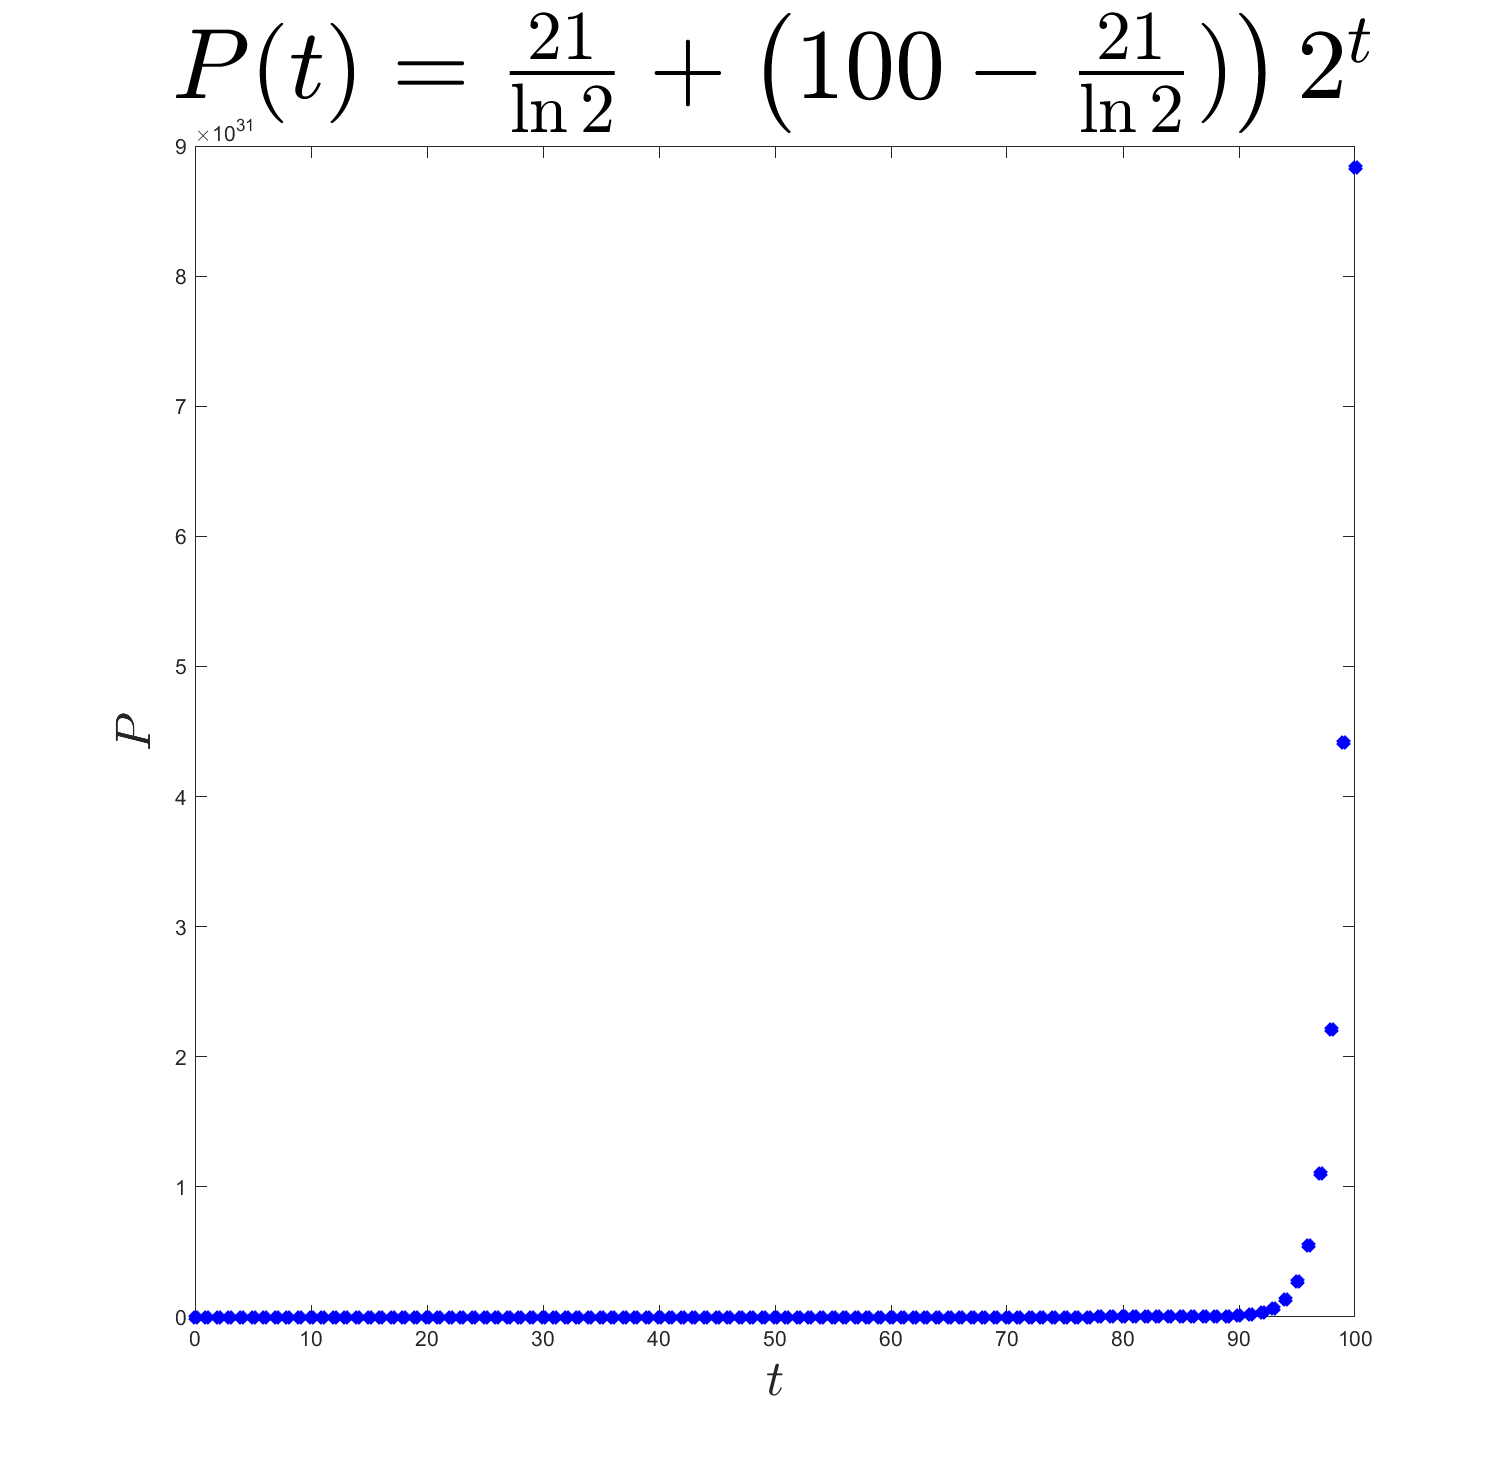
\includegraphics[width=0.75\textwidth]{PS3_fig1.png}
\end{center}
It seems that the beatle population will survive. According to our model, $P(100)\approx 8.8\times10^{31}$. Which means, after 100 weeks, a little under 2 years, the Christmas beetle population in Brisbane is predicted to weigh $8.8\times10^{27}$kg, about 4.5 times heavier then the planet Jupiter.

\pagebreak
\sol (d) We will plot our solution, but with inital population ranging between from $P_0=20$ to $P_0=50$.\\
\verb|PS3_script2.m| \hrule
\begin{lstlisting}{Matlab}
hold on;
for inital_pop = 20:1:50
	P = @(t) (21/log(2)) + (inital_pop - (21/log(2)))*2.^t;
	t = 0:1:100;
	y = P(t);
	plot(t,y, 'r',  "LineWidth", 1);
end

title("$P(t) = \frac{21}{\ln2} + \left( P_0 - \frac{21}{\ln2}) \right)2^t$"...
	, "Interpreter", "latex", "FontSize", 48);
xlabel("$t$", "FontSize", 24, "Interpreter", "latex");
ylabel("$P$", "FontSize", 24, "Interpreter", "latex");
\end{lstlisting}
\verb|Output:|\\
\begin{center}
	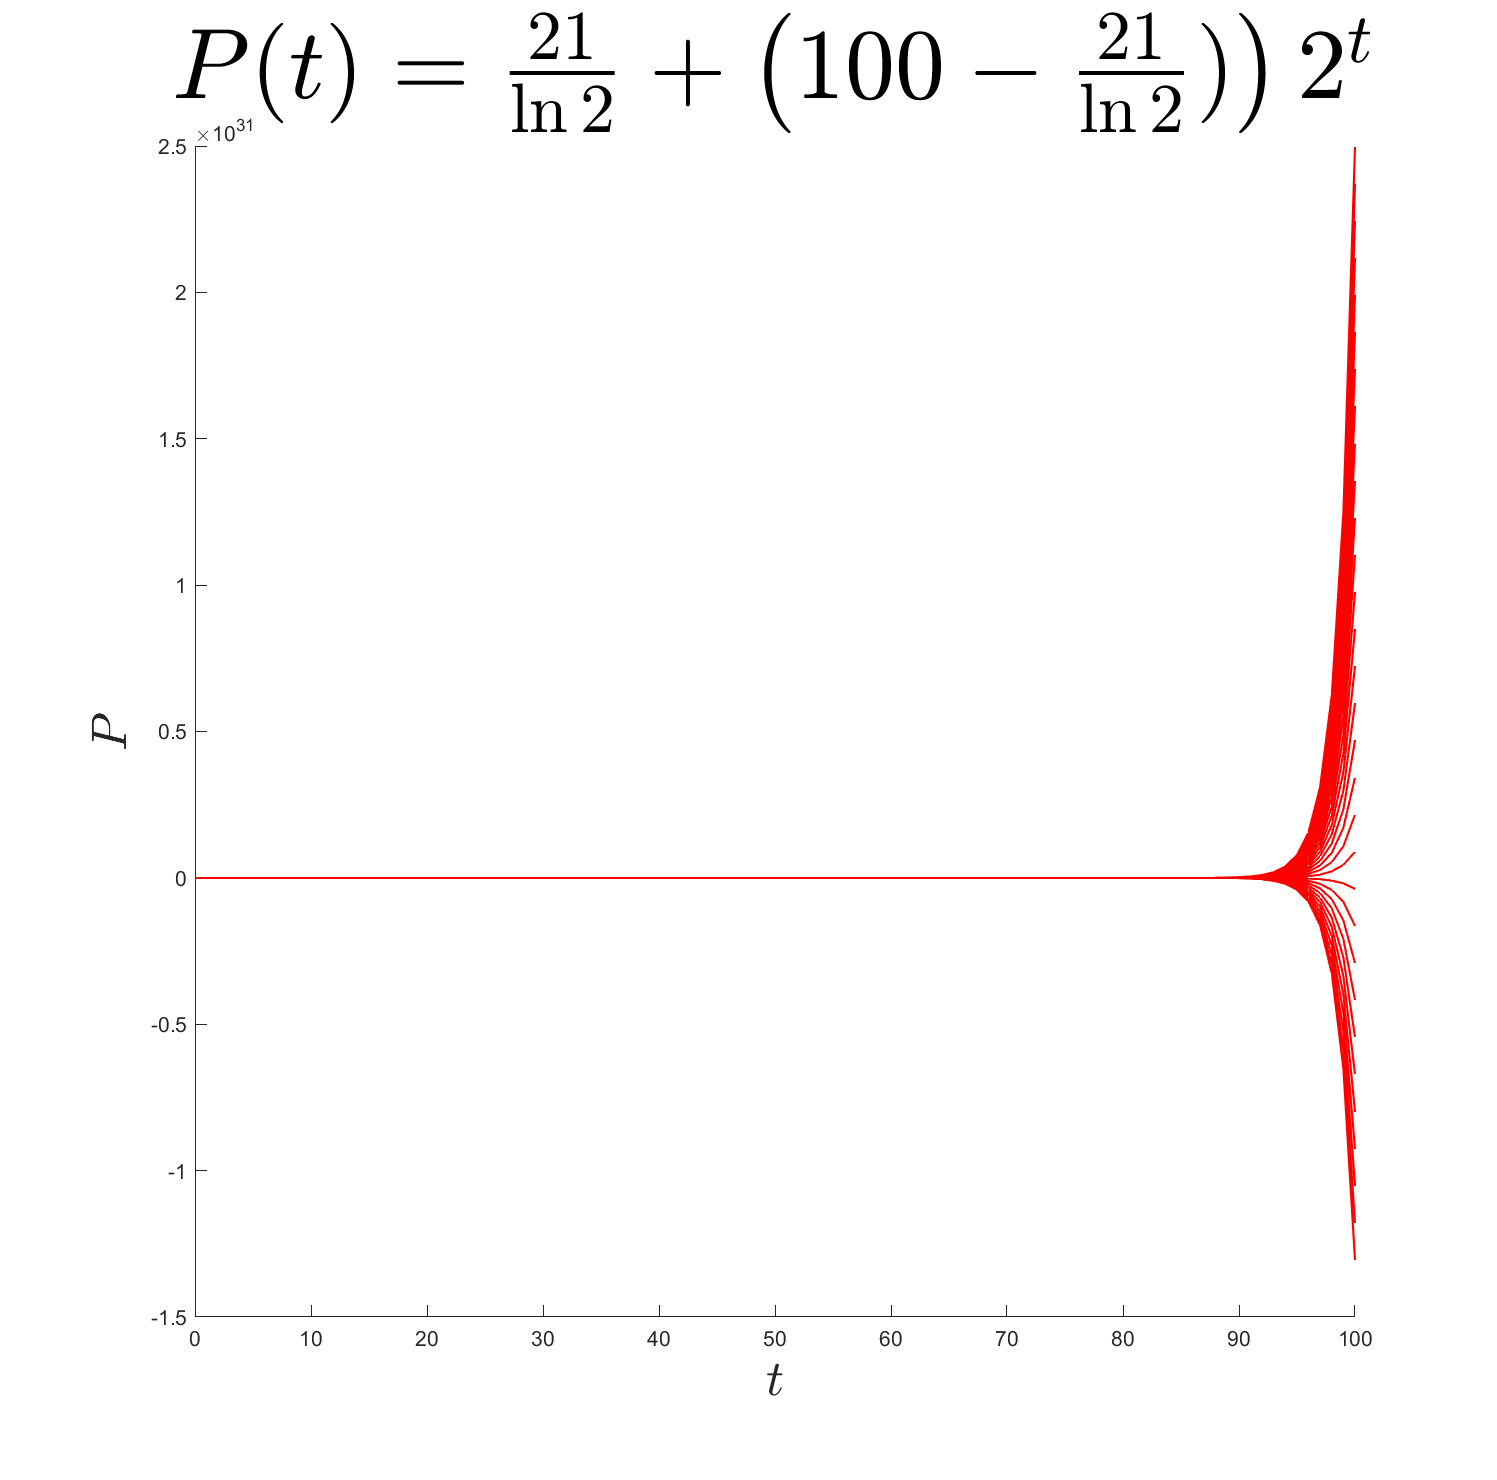
\includegraphics[width=0.75\textwidth]{PS3_fig2.png}
\end{center}
We can clearly see that there is an unstable equilibrium! In fact, upon analysis of the ODE, we can conclude that there is an equilibrium when $p_0=21/\ln2$, and confirm this:
$$
	P(t) = \frac{21}{\ln2} + \bracks{\frac{21}{\ln2} - \frac{21}{\ln2}}2^t = \frac{21}{\ln2} \implies \dyd[P]{t}=0,\ \forall t
$$
Of course, the inital population must be an integer, and so could never truly equal $21/\ln2$ initally, but the equilibrium is still there, theoretically.

\newpage
\qs{Fluid Flow}{
	In this question, we take the cartesian variables as $x\equiv x_1,$ $y\equiv x_2,$ and $z\equiv x_3.$ We also take the basis vectors as $\ihat\equiv\ut{e}_1$, $\jhat\equiv\ut{e}_2,$ and $\khat\equiv\ut{e}_3$. \\
	
	In fluid mechanics, fluids which are \textbf{incompressible} and \textbf{inviscid} are referred to as \textbf{ideal}.
	
	Let $\ut{u}=\ut{u}(x,y,z,t)=u_1\ut{e}_1+u_2\ut{e}_2+u_3\ut{e}_3$ be the velocity of an ideal fluid at an arbitrary point in space and time. Its motion is governed by the Euler equation,
	$$
		\del{\ut{u}}{t} + (\ut{u}\cd\nabla)\ut{u} =\ut{F} - \frac{\nabla P}{\rho}.
	$$
	Here $P$ is the fluid's pressure, $\rho$ its constant density, $\ut{F}$ is the external force on the fluid at any given point, and
	$$
		(\ut{u}\cd\nabla)\ut{u} \equiv \sum_{i=1}^3 u_i\del{\ut{u}}{x_i}.
	$$
	Suppose the system is simplified in three ways:
	\begin{itemize}
		\item The flow is \textbf{steady}. $\ut{u}=\ut{u}(x,y,z)$ is not changing with time.
		\item $\ut{u}$ is a conservative vector field. This occurs when the fluid is \textbf{irrotational}, though we won't elaborate on that here.
		\item The external force is also conservative, with $\ut{F}=-\nabla V$, for some scalar potential $V = V(x_1,x_2,x_3)$.  
	\end{itemize}
	
	\begin{enumerate}[label=(\alph*)]
		\item Show that in this case, 
		$$
			(\ut{u}\cdot\nabla)\ut{u}=\frac{1}{2}\nabla ||\ut{u}||^2.
		$$ (Hint, you can assume that Clairaut's theorem applies)
		\item Hence show that the Euler equation simplifies to
		$$
			\frac{1}{2}||\ut{u}||^2+V+\frac{P}{\rho}=\text{constant}
		$$
		\item If $V$ is a constant, what can you say about the relationship between a fluid's speed and its pressure?
	\end{enumerate}
}
\sol (a)
We seek to show that $(\ut{u}\cd\grad)\ut{u} = \frac{1}{2}\grad\Mag{\ut{u}}^2$.
\proof
\begin{align*}
	\ut{u} &= u_1\ut{e}_1 + u_2\ut{e}_2 + u_3\ut{e}_3 \\
	\iff\Mag{\ut{u}} &= \sqrt{u_1^2 + u_2^2 + u_3^2} \\
	\iff\Mag{\ut{u}}^2 &= u_1^2 + u_2^2 + u_3^2 \\
	\iff\grad\Mag{\ut{u}}^2 &= \grad\bracks{u_1^2 + u_2^2 + u_3^2} \\
		&= \bracks{\del{}{x_1}\ut{e_1} + \del{}{x_2}\ut{e_2} + \del{}{x_3}\ut{e_3}}\bracks{u_1^2 + u_2^2 + u_3^2} \\
		&= \del{\bracks{u_1^2 + u_2^2 + u_3^2}}{x_1}\ut{e_1} + \del{\bracks{u_1^2 + u_2^2 + u_3^2}}{x_2}\ut{e_2} + \del{\bracks{u_1^2 + u_2^2 + u_3^2}}{x_3}\ut{e_3} \\
	\intertext{We'll take the partial derivatives. $u_j$ is zeroed by $x_i$ if $i\neq j$. And since $u_i$ are functions of $x_i$, they are chain ruled}
	\grad\Mag{\ut{u}}^2 &= 2u_1\del{u_1}{x_1}\ut{e_1} + 2u_2\del{u_2}{x_2}\ut{e_2} + 2u_3\del{u_3}{x_3}\ut{e_3} \\
		&= 2\bracks{u_1\del{u_1}{x_1}\ut{e_1} + u_2\del{u_2}{x_2}\ut{e_2} + u_3\del{u_3}{x_3}\ut{e_3}} \\
	\tf LHS=\frac{1}{2}\grad\Mag{\ut{u}}^2 &= u_1\del{u_1}{x_1}\ut{e_1} + u_2\del{u_2}{x_2}\ut{e_2} + u_3\del{u_3}{x_3}\ut{e_3} \\
		&= \sum_{i=1}^{3} \bracks{u_i\del{u_i}{x_i}\ut{e_i}} \\
		&= \sum_{i=1}^{3} \bracks{u_i\del{\ut{u}}{x_i}} \\
		&= (\ut{u}\cd\grad)\ut{u} = RHS \tag*{\qed}
\end{align*}

\sol (b) We will start by taking the Euler equation, as in the question box above, and substituting the result we proved in (a)
\begin{gather*}
	\del{\ut{u}}{t} + (\ut{u}\cd\nabla)\ut{u} =\ut{F} - \frac{\nabla P}{\rho} \\
	\iff \del{\ut{u}}{t} + \frac{1}{2}\grad\Mag{\ut{u}}^2 =\ut{F} - \frac{\nabla P}{\rho}
	\intertext{Next, since the external force is conservative, we'll substitute $\ut{F}=-\grad V$, where $V$ is some scalar potential.}
	\iff \del{\ut{u}}{t} + \frac{1}{2}\grad\Mag{\ut{u}}^2 =-\grad V - \frac{\nabla P}{\rho} \\
	\iff \frac{1}{2}\grad\Mag{\ut{u}}^2 + \grad V + \frac{\nabla P}{\rho} =- \del{\ut{u}}{t}
	\intertext{Now, since the flow is steady, $\dyd[\ut{u}]{t}=0$}
	\iff \frac{1}{2}\grad\Mag{\ut{u}}^2 + \grad V + \frac{\grad P}{\rho} = 0
	\intertext{Finally, we'll take out the $\grad$}
	\iff \grad\bracks{\frac{1}{2}\Mag{\ut{u}}^2 + V + \frac{P}{\rho}} = 0
	\intertext{The gradient of a function can only be $0$ if the function itself is equal to some constant. Thus we've shown that, under these conditions, the Euler equation simplies to}
	\frac{1}{2}\Mag{\ut{u}}^2 + V + \frac{P}{\rho} = \text{constant}
\end{gather*}

\sol (c) If $V$ is constant, we can simplify the model.
$$
	\frac{1}{2}\Mag{\ut{u}}^2 + \frac{P}{\rho} = C
$$
where $C$ is some constant. \\

The two remaining terms are related in a such a way that, if fluid speed, $\Mag{\ut{u}}$, were to increase, then the pressure, $P$, must decrease to compenstate, and keep the sum equal to the constant $C$; and vice versa. Thus, if $V$ is constant, there is an inverse relationship between the speed of an ideal fluid and its pressure.


\newpage
\qs{First Order Differential Equation}{
	Consider Newton's second law of motion which states that,
	\[ 
		F = ma \tag{1}\label{eq:newtonsecond}
	\]
	or: net force, $F$, is equal to mass $m$, times acceleration $a$.
	\begin{enumerate}[label=(\alph*)]
		\item Use equation \eqref{eq:newtonsecond} to write out the equation of motion of a particle of mass $m$, subject to a frictional force proportional to the square of the velocity $v(t)$, completely in terms of the particle's velocity $v(t)$.
		\item Solve the first-order differential equation from part (a) to find the particle's velocity $v(t)$ at time $t$, with initial velocity $v_0$.
		\item Use your solution from part (b) to solve for the position of the particle $x(t)$ at time $t$, with initial position $x_0$.
		\item Use Euler's method with step size 0.1 to estimate the particle's position $x(0.5)$ at time $t = 0.5$ of your solution in part (b). Take $m = 1$, $k = 2$, $x_0 = 0$, and $v_0 = 1$. Calculate the error in using Euler's method, rounded to the fourth decimal.
	\end{enumerate}
}
\sol (a) Suppose a particle has mass $m$ and velocity $v$, which is itself a funciton of time $t$. Acceleration is just the derivative of velocity with respect to time, thus, the net force acting on it, can be expressed
$$
	F = m\dyd[v]{t}
$$
Next, we consider the frictional force, $F_\text{f}$, which is proportaional to the velocity squared. Let $k$ be the constant of proportionality.
$$
	F_{\text{f}} = -kv^2
$$
The sign is negative because friction acts against the motion of the particle. The only force acting on the particle, which means, by Newton's Second Law, net forces cancel out.
$$
	F - F_{\text{f}} = 0 \iff F = F_{\text{f}}
$$
Subsituting the $F$'s in terms of $v$'s,
$$
	m\dyd[v]{t} = -kv^2
$$
Rearranging,
$$
	\dyd[v]{t} = -\frac{k}{m}v^2
$$

\sol(b) We can start by noting that the ODE has an equilibrium when
$$
	v=0 \implies \dyd[v]{t},\ \forall t
$$
$v=0$ is a singular solution to the ODE. \\
We will now proceed with the restriction $v\neq 0$. \\
This ODE is seperable, that is, it can be expressed
$$
	\dyd[v]{t} = f(t)g(v)
$$
In our case, 
$$
	f(t) = -\frac{k}{m},\qquad g(v) = v^2
$$
From this position, we can start to find the general solution.
\begin{align*}
	\dyd[v]{t} &= f(t)g(v) \\
	\frac{1}{g}\dyd[v]{t} &= f(t) \\
	\int\frac{1}{g}\dyd[v]{t}\d t &= \int f(t)\d t \\
	\int v^{-2}\d v &= \int -\frac{k}{m} \d t \\
	\frac{-1}{v} + c_1 &= -\frac{k}{m} \int \d t \\
		&= -\frac{k}{m}t + c_2 \\
	\frac{1}{v} &= \frac{k}{m}t + \hat{c},\ (\hat{c} = c_1 - c_2)\in\bbr \\
	\tf v &= \frac{1}{\frac{k}{m}t + \hat{c}} \\
		&= \frac{m}{kt + \hat{c}m}
\end{align*}
Now, we'll solve for $\hat{c}$, given our inital condition, $v(0)=v_0$
\begin{align*}
	v(0) = v_0 &= \frac{m}{k(0) + \hat{c}m} \\
	\hat{c}m &= \frac{m}{v_0} \\
	\hat{c} &= \frac{1}{v_0}
\end{align*}
Next, we'll subtitute this back into our general solution.
$$
	v(t) = \frac{m}{kt + \frac{1}{v_0}m}
$$
Finally, we'll simplify and present the particular solution to the ODE
$$
	v(t) = \frac{mv_0}{kv_0t + m}
$$

\sol (c) Position, $x(t)$ can be found by integrating velocity with respect to $t$.
$$
	x(t) = \int v(t)\d x = \int \frac{mv_0}{kv_0t + m}\d t = \frac{mv_0}{kv_0}\ln\abs{kv_0 t + m} + \hat{c} = \frac{m}{k}\ln\abs{kv_0 t + m} + \hat{c} 
$$
We'll use the inital condition $x(0)=x_0$ to solve for $c$,
$$
	x(0) = x_0 = \frac{m}{k}\ln\abs{kv_0(0) + m} + \hat{c} = \frac{m}{k}\ln\abs{m}+\hat{c} \iff \hat{c} = x_0 - \frac{m}{k}\ln\abs{m} 
$$
Substituting back in,
$$
	x(t) = \frac{m}{k}\ln\abs{kv_0 t + m} + x_0 - \frac{m}{k}\ln\abs{m} = \frac{m}{k}\bracks{\ln\abs{kv_0t + m} - \ln\abs{m}} + x_0
$$
Which means the final solution for position is
$$
	x(t) = x_0 + \frac{m}{k}\ln\abs{\frac{kv_0t + m}{m}}
$$

\sol (d) Euler's method states (with notation adapted for this specific problem)
$$
	x_{n+1} = x_{n} + f(t_{n}, v_{n})\D t
$$
Given $\D t =0.1$ and $x'(t) = f(t_n, v_n) = v(t)$, we can write
$$
	x_{n+1} = x_{n} + 0.1\frac{v_0m}{m+kv_0t_n}
$$
Taking $m=1$, $k=2$, $x_0=0$ and $v_0=1$, we can write our solution, and Euler method as
$$
	v(t) = \frac{1}{2t + 1},\qquad x_{n+1} = x_{n} + \frac{1}{10+20t_n}
$$
Now, given $\D t = 0.1$, the $t$ values we're interested in are 
$$
	t_0 = 0,\qquad t_1 = 0.1,\qquad t_2 = 0.2,\qquad t_3 = 0.3,\qquad t_4 = 0.4,\qquad t_5 = 0.5 
$$
We are no ready to make our Euler method itterations
\begin{gather*}
	t_0 = 0.0: x_0 = 0 \tag*{(\text{Given})} \\
	t_1 = 0.1: x_1 = x_0 + \frac{1}{10+20t_0} = 0 + \frac{1}{10+20(0.0)} = \frac{1}{10} = 0.1 \\
	t_2 = 0.2: x_2 = x_1 + \frac{1}{10+20t_1} = \frac{1}{10} + \frac{1}{10+20(0.1)} = \frac{11}{60} \approx 0.1833 \\
	t_3 = 0.3: x_3 = x_2 + \frac{1}{10+20t_2} = \frac{11}{60} + \frac{1}{10+20(0.2)} = \frac{107}{420} \approx 0.2548 \\
	t_4 = 0.4: x_4 = x_3 + \frac{1}{10+20t_3} = \frac{107}{420} + \frac{1}{10+20(0.3)} = \frac{533}{1680} \approx 0.3173 \\
	t_5 = 0.5: x_5 = x_4 + \frac{1}{10+20t_4} = \frac{533}{1680} + \frac{1}{10+20(0.4)} = \frac{1879}{5040} \approx 0.3728 \\
\end{gather*}
Therefore, using Euler's Method, we find that $x(0.5)\approx 0.3728$. \\
Let's now find the exact value of $x(0.5)$. We will use the $x(t)$ we found eariler, and substitute the fixed $m$, $k$, $x_0$, and $v_0$.
$$
	x(0.5) = \frac{1}{2}\ln\abs{2(0.5) + 1} = \frac{1}{2}\ln2 \approx 0.3466
$$
Finally, let's find the error. Let $\bar{x}$ be the value calcualted using Euler's method, and let $x$ be the true position of the particle. 
$$
	\veps = \abs{x(0.5) - \bar{x}(0.5)} = \abs{\frac{1}{2}\ln2 - \frac{1879}{5040}} \approx 0.0262
$$


\newpage
\qs{Line Integral}{
	Evaluate the line integral
	$$
		\int_C x e^y\ \d{s},
	$$
	where $C$ is the line segment from $(2,0)$ to $(5,4)$.
}
\sol
\begin{gather*}
	\longintertext{Our first goal will be to find some $\ut{r}(t)$ which correctly expresses the path $C$. \\ First, we note that when $t=0,\ \ut{r}=(2,0)$. \\ Second, we note that at $t=1,\ \ut{r}=(5,4)$. \\ Since, this is path is a straight line, we can use a linear interpolation,}
	\begin{aligned}
		\ut{r}(t) &= \bracks{x(t), y(t)} \\
			&= \bracks{x_0 + t\D x, y_0 + t\D y}	\\
			&= \bracks{2 + t(5-2), 0 + t(4-0)} \\
			&= \bracks{3t + 2, 4t}
	\end{aligned}
	\intertext{Next, we should find the derivative of $\ut{r}$ with respect for $t$.}
	\begin{aligned}
		\dyd[\ut{r}]{t} &= \bracks{\dd{t}\bracks{3t+2}, \dd{t}\bracks{4t}} \\
			&= \bracks{3, 4}
	\end{aligned}
	\intertext{Finally, we'll find the magnitude of the derivative.}
	\abs{\abs{\dyd[\ut{r}]{t}}}	= \sqrt{3^2 + 4^2} 
		= \sqrt{9 + 16} 
		= \sqrt{25} 
		= 5
	\intertext{We note that}
	\d s = \abs{\abs{\dyd[\ut{r}]{t}}}\d t = 5\d t
	\intertext{and proceed to make the subsitutions into the line integral we seek to evaluate}
	\begin{aligned}
		\int_C x\exp(y)\ \d s &= \int_{0}^{1} x(t)\exp(y(t))5\ \d t \\
			&= \int_0^1 5(3t+2)\exp\bracks{4t}\ \d t \\
			&= 5\int_0^1 (3t+2)\exp\bracks{4t}\ \d t \\
			&= 5\bracks{2\int_0^1 \exp\bracks{4t} \d t + 3\int_0^1 t\exp\bracks{4t} \d t} \\
			&= 5\bracks{2A + 3B}
	\end{aligned}
	\intertext{Let's first evaluate the integral $A$, we'll use a $u{-}$substitution and the identity $f'(x)=\exp(x)=f(x)$.}
	\begin{aligned}
		A &= \int_0^1 \exp(4t)\d t \\
		\Let u &= 4t \\
		\Then \dyd[u]{t} &= 4 \implies \d t = \frac{1}{4}\d u \\
		\tf A &= \frac{1}{4}\int_{4\cd0}^{4\cd1} \exp(u)\d u \\
			&= \left. \frac{1}{4}\cd \exp(u) \right|_{0}^{4} \\
			&= \frac{1}{4}\bracks{\exp(4) - \exp(0)} \\
		\tf A = \int_0^1 \exp(4t)\d t &= \frac{1}{4} \bracks{\exp(4) - 1}
	\end{aligned}
	\intertext{Next, let's evaluate the integral $B$, where we'll use integration by parts, and the previous result.}
	\begin{align*}
		B &= \int_0^1 t\exp(4t)\d t \\ 
			&= \int_0^1 uv'\d t \\
			&= \left. uv \right|_0^1 - \int_0^1 u'v\d t \\
		u = t &\Rightarrow u' = 1 \\
		v' = \exp(4t) &\Rightarrow v = \frac{1}{4}\exp(4t) \\
		\left. uv \right|_0^1 - \int_0^1 u'v\d t &= \left. t\frac{1}{4}\exp(4t) \right|_0^1 - \int_0^1 1\cd\frac{1}{4}\exp(4t)\d t \\
			&= \frac{1}{4}\bracks{1\exp(4\cd1) - 0\exp(4\cd0)} - \frac{1}{4}\int_0^1\exp(4t)\d t \\
			&= \frac{1}{4}\exp(4) - \frac{1}{4}\bracks{\frac{1}{4}\bracks{\exp(4)-1}} \tag*{(\text{Previous Result})} \\
			&= \frac{4}{16} \exp(4) - \frac{1}{16}\exp(4) + \frac{1}{16} \\
		\tf B = \int_0^1 t\exp(4t)\d t &= \frac{3}{16}\exp(4) + \frac{1}{16}
	\end{align*}
	\intertext{Let's bring it all together now}
	\begin{aligned}
		\int_C x\exp(y)\ \d s &= 5(2A + 3B) \\
			&= 5\bracks{2\bracks{\frac{1}{4} \bracks{\exp(4) - 1}} + 3\bracks{\frac{3}{16}\exp(4) + \frac{1}{16}}} \\
			&= 5\bracks{\bracks{\frac{1}{2} \bracks{\exp(4) - 1}} + \frac{9}{16}\exp(4) + \frac{3}{16}} \\
			&= 5\bracks{\frac{8}{16}\exp(4) + \frac{9}{16}\exp(4) + \frac{3}{16} - \frac{8}{16}} \\
			&= 5\bracks{\frac{17}{16}\exp(4) - \frac{5}{16}} \\
		\tf\int_C x\exp(y)\d s &= \frac{85}{16}\exp(4) - \frac{25}{16} \approx 288.4902
	\end{aligned}
\end{gather*}

\end{document}
